\section{Zeichnen mit Tikz}

\begin{frame}[fragile]{%
  Ti\textit{k}Z
  \hfill
  \doc{http://mirrors.ctan.org/graphics/pgf/base/doc/pgfmanual.pdf}{tikz/pgf}
}
  \begin{Packages}
    \mintinline{latex}+\usepackage{tikz}+
  \end{Packages}
  \begin{itemize}
    \item \alert{T}i\textit{k}z \alert{i}st \alert{k}ein \alert{Z}eichenprogramm
    \item Zeichnen mit Befehlen
      \begin{itemize}
        \item Sehr präzise (Kleinste Einheit in \TeX ${} \approx \qty{5}{\nano\meter}$)
        \item programmierfähig
        \item automatisierbar
        \item Versionskontrolle!
      \end{itemize}
    \item Extrem umfangreiche Doku mit \emph{zahlreichen} Beispiel (>\num{1000} Seiten)
    \item Basis-Einheit ist \unit{\centi\meter}
  \end{itemize}
  \begin{CodeExample}{0.7}
    \begin{minted}{latex}
      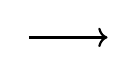
\begin{tikzpicture}
        \draw[thick, ->] (0, 0) -- (1, 0);
      \end{tikzpicture}
    \end{minted}
  \CodeResult
  \strut\\
    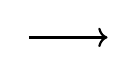
\begin{tikzpicture}
      \draw[thick, ->] (0, 0) -- (1, 0);
    \end{tikzpicture}
  \end{CodeExample}
\end{frame}
\begin{frame}[fragile]{Kleine Beispiele}
  \begin{CodeExample}{0.8}[\texttt{cycle}]
    \begin{minted}{latex}
      
\begin{tikzpicture}
        \draw[thick] (0, 0) -- (1, 0) -- (1, 1) -- cycle;
      \end{tikzpicture}
    \end{minted}
  \CodeResult
    
\begin{tikzpicture}
        \draw[thick] (0, 0) -- (1, 0) -- (1, 1) -- cycle;
    \end{tikzpicture}
  \end{CodeExample}
  \begin{CodeExample}{0.8}[Polarkoordinaten]
    \begin{minted}{latex}
      
\begin{tikzpicture}
        \foreach\ang in {0, 45, 90, 135, 180, 215, 270, 315}
        {
          \draw (0, 0) -- (\ang: 10pt);
        }
      \end{tikzpicture}
    \end{minted}
  \CodeResult
    
\begin{tikzpicture}
      \foreach\ang in {0, 45, 90, 135, 180, 215, 270, 315}
      {
        \draw (0, 0) -- (\ang: 10pt);
      }
    \end{tikzpicture}
  \end{CodeExample}
\end{frame}

\begin{frame}[fragile]{Kleine Beispiele}
  \begin{CodeExample}{0.8}[\texttt{nodes}]
    \begin{minted}{latex}
      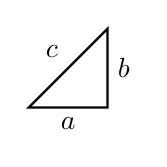
\begin{tikzpicture}
        \draw[thick] (0, 0)
          -- (1, 0) node[midway, below] {$a$}
          -- (1, 1) node[midway, right] {$b$}
          -- cycle  node[midway, above left] {$c$};
      \end{tikzpicture}
    \end{minted}
  \CodeResult
    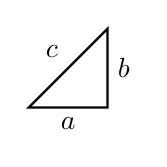
\begin{tikzpicture}
      \draw[thick] (0, 0)
        -- (1, 0) node[midway, below] {$a$}
        -- (1, 1) node[midway, right] {$b$}
        -- cycle  node[midway, above left] {$c$};
    \end{tikzpicture}
  \end{CodeExample}
\end{frame}

\begin{frame}[fragile]{Tikz-Feynman}
  \begin{Packages}
    \mintinline{latex}+\usepackage{tikz-feynman}+
  \end{Packages}
  \begin{CodeExample}{0.65}[Tree-Graph]
    \begin{minted}{latex}
      \feynmandiagram [horizontal=a to b] {
        i1 -- [fermion] a -- [fermion] i2,
        a -- [photon] b,
        f1 -- [fermion] b -- [fermion] f2,
      };
    \end{minted}
  \CodeResult
    \feynmandiagram [horizontal=a to b] {
      i1 -- [fermion] a -- [fermion] i2,
      a -- [photon] b,
      f1 -- [fermion] b -- [fermion] f2,
    };
  \end{CodeExample}
\end{frame}

\begin{frame}[fragile]{Tikz-Feynman}
  \begin{CodeExample}{0.65}[Tree-Graph]
    \begin{minted}{latex}
      \feynmandiagram [horizontal=a to b] {
        i1 [particle=$\symup{e}^-$]
          -- [fermion] a
          -- [fermion] i2 [particle=$\symup{e}^+$],
        a -- [photon, edge label=$\symup{γ}$] b,
        f1 [particle=$\symup{μ}^-$]
          -- [fermion] b
          -- [fermion] f2 [particle=$\symup{μ}^+$],
      };
    \end{minted}
  \CodeResult
    \feynmandiagram [horizontal=a to b] {
      i1 [particle=$\symup{e}^-$] -- [fermion] a -- [fermion] i2 [particle=$\symup{e}^+$],
      a -- [photon, edge label=$\symup{γ}$] b,
      f2 [particle=$\symup{μ}^+$] -- [fermion] b -- [fermion] f1 [particle=$\symup{μ}^-$],
    };
  \end{CodeExample}
\end{frame}
